\documentclass[11pt]{article}
 
\usepackage[margin=1in]{geometry} 
\usepackage{amsmath,amsthm,amssymb}
\usepackage[margin=1in]{geometry} 
\usepackage{amsmath,amsthm,amssymb}
\usepackage[spanish]{babel} %Castellanización
\usepackage[T1]{fontenc} %escribe lo del teclado
\usepackage[utf8]{inputenc} %Reconoce algunos símbolos
\usepackage{lmodern} %optimiza algunas fuentes
\usepackage{graphicx}
\graphicspath{ {images/} }
\usepackage{hyperref} % Uso de links
\usepackage{minted}

\usepackage{listings}
\usepackage{color}
\usepackage[dvipsnames,table]{xcolor}
\usepackage{forest}
\usepackage{float}
\usepackage{empheq}

\usepackage{tikz}
\usetikzlibrary{calc,shapes.multipart,chains,arrows}
\def\checkmark{\tikz\fill[scale=0.4](0,.35) -- (.25,0) -- (1,.7) -- (.25,.15) -- cycle;} 

\definecolor{codegreen}{rgb}{0,0.6,0}
\definecolor{codegray}{rgb}{0.5,0.5,0.5}
\definecolor{codebrown}{rgb}{0.75,0.1,0.3}
\definecolor{backcolour}{rgb}{0.95,0.95,0.92}
 
\lstdefinestyle{mystyle}{
    backgroundcolor=\color{backcolour},   
    commentstyle=\color{codegreen},
    keywordstyle=\color{magenta},
    numberstyle=\tiny\color{codegray},
    stringstyle=\color{codebrown},
    basicstyle=\footnotesize,
    breakatwhitespace=false,         
    breaklines=true,                 
    captionpos=b,                    
    keepspaces=true,                 
    numbers=left,                    
    numbersep=5pt,                  
    showspaces=false,                
    showstringspaces=false,
    showtabs=false,                  
    tabsize=2
}

\lstset{style=mystyle}

\newcommand{\N}{\mathbb{N}}
\newcommand{\Z}{\mathbb{Z}}
 
\newenvironment{theorem}[2][Theorem]{\begin{trivlist}
\item[\hskip \labelsep {\bfseries #1}\hskip \labelsep {\bfseries #2.}]}{\end{trivlist}}
\newenvironment{lemma}[2][Lemma]{\begin{trivlist}
\item[\hskip \labelsep {\bfseries #1}\hskip \labelsep {\bfseries #2.}]}{\end{trivlist}}
\newenvironment{exercise}[2][Exercise]{\begin{trivlist}
\item[\hskip \labelsep {\bfseries #1}\hskip \labelsep {\bfseries #2.}]}{\end{trivlist}}
\newenvironment{problem}[2][Problem]{\begin{trivlist}
\item[\hskip \labelsep {\bfseries #1}\hskip \labelsep {\bfseries #2.}]}{\end{trivlist}}
\newenvironment{question}[2][Question]{\begin{trivlist}
\item[\hskip \labelsep {\bfseries #1}\hskip \labelsep {\bfseries #2.}]}{\end{trivlist}}
\newenvironment{corollary}[2][Corollary]{\begin{trivlist}
\item[\hskip \labelsep {\bfseries #1}\hskip \labelsep {\bfseries #2.}]}{\end{trivlist}}

\newenvironment{solution}{\begin{proof}[Solution]}{\end{proof}}

\begin{document}

\title{\textbf{ Práctica 3: Intérprete para un lenguaje P}}
\author{
        Iván López de Munain Quintana\\ \\
\textit{Gramáticas y Lenguajes Formales}}

\maketitle

\vspace{50px}
\begin{center}
    
\includegraphics[width=300px, height=300px]{escudo_uva.png}    
\end{center}

\newpage

\setcounter{tocdepth}{2}
\tableofcontents


\newpage

\noindent Los objetivos de esta práctica son afianzar los conceptos aprendidos sobre las herramientas \textit{Lex} y \textit{Yacc} para la construcción de analizadores sintácticos y léxicos. Básicamente se pretende construir un intérprete de un lenguaje (P) que es similar al lenguaje C. Cabe remarcar que a la hora de realizar los siguiente apartados he utilizado como ficheros base los realizados por el profesor Dusan Kolár \footnotemark en la exposición que realizó para el alumnado.

\footnotetext{Profesor de la Universidad de Brno (Chequia) }

\section{Especificaciones léxicas}

\noindent En este apartado se va a describir los elementos léxicos del lenguaje P, todos ellos van a ser descritos mediante expresiones regulares en el fichero llamado \textit{pcc.l}.

\subsection{Identificadores y palabras claves}

\noindent Los identificadores se definen mediante un conjunto de letras, números, '\_' tal que comiencen por '\_' o por una letra. Esto se consiguie con la siguiente expresión regular. 

\begin{minted}{bash}
    LETTER    ([_a-zA-Z])
    IDENT     (("_")*{LETTER}({LETTER}|{DIGIT})*)
\end{minted}


\noindent Siendo \textit{IDENT} el correspondiente identificador.

\subsection{Constantes numéricas}

\noindent Este tipo de elementos poseen una parte entera que puede ir seguida de una parte decimal, además podrán expresarse en notación decimal (representándose el exponente mediante 'E' o 'e' seguido del signo '-' o '+'). Esto se consigue en el fichero \textit{pcc.l} a través de las expresiones regulares siguientes: \\

\begin{minted}{bash}
    DIGIT     ([0-9])
    DIGITS    ({DIGIT}+)
    
    EXP       ([eE][-+]?{DIGITS})
    
    FLOAT1    ({DIGITS}"."{DIGITS})
    FLOAT2    ({DIGITS}{EXP})
    FLOAT3    ({DIGITS}"."{DIGITS}{EXP})
    
    FLOAT    ({FLOAT1}|{FLOAT2}|{FLOAT3})

\end{minted}
\\

\newpage

\noindent Posteriormente para realizar su almacenamiento en el formato pedido (coma flotante de doble precisión o double) bastará con implementar lo siguiente en la parte intermedia del archivo \textit{Lex}. \\

\begin{figure}[H]
  \centering
    \fbox{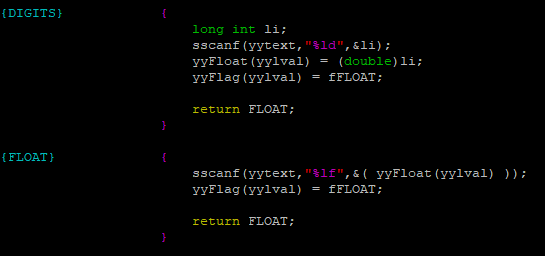
\includegraphics[width=0.65\textwidth]{numericos.PNG}}
  \caption{Acción al encontrarse constantes numéricas.}
\end{figure}

\subsection{Constantes carácter y tiras de caracteres}

\noindent Tan solo se han implementado las tiras de caracteres, no operaciones que las utilicen.

\begin{minted}{bash}

    STRSTART  (["])

\end{minted}

\%\%
\begin{minted}{bash}
    {STRSTART}          {
                      yyStr(yylval) = readStr();
                      yyFlag(yylval) = fSTR;

                      return STR;
                    }
\end{minted}


\subsection{Separadores}

\noindent Para realizar este apartado tenemos que tener en cuenta que los espacios en blanco, tabuladores (\textit{$\textbackslash t$}), saltos de línea (\textit{$\textbackslash n$}), salto de carro (\textit{ $\textbackslash r$}) y form feed (\textit{$\textbackslash f$}).

\begin{minted}{bash}
    EOL    ([\n])
    
    WSPC      ([\t\f\r])
    WSPCS     ({WSPC}+)

\end{minted}

\newpage

\noindent Como en estas ocasiones no queremos que el intérprete haga nada, simplemente les ignore tan solo tendremos que añadir lo siguiente en la parte intermedia de \textit{pcc.l}:

\begin{minted}{bash}

{EOL}            {
                        ++yylineno;
                        return EOL;
                    }


{WSPC}              ;  /* nada que hacer, espacio en blanco */


\end{minted}

\noindent Cabe destacar que para indicar los bloques de las secciones a través de llaves se hace de la misma forma.


\subsection{Comentarios}

\noindent Pese a que en el enunciado de la práctica dice que tan solo hay que implementar un intérprete que ignore los comentarios de una línea (no permitiendo los multilínea), voy a implementar que ignore los multilínea pues el otro caso es un caso específico de este. Para el caso de comentario multilína cada vez que se encuentre el patrón \textit{$"/*"$} se ejecutará el método \textit{IgnoraComentarioMultiLinea(&nlin, &ncol)}:

\begin{minted}{bash}

    "/\*"   IgnoraComentarioMultiLinea(&nlin, &ncol);

\end{minted}

\noindent Siendo el código de dicho método el siguiente: \\

\begin{figure}[H]
  \centering
    \fbox{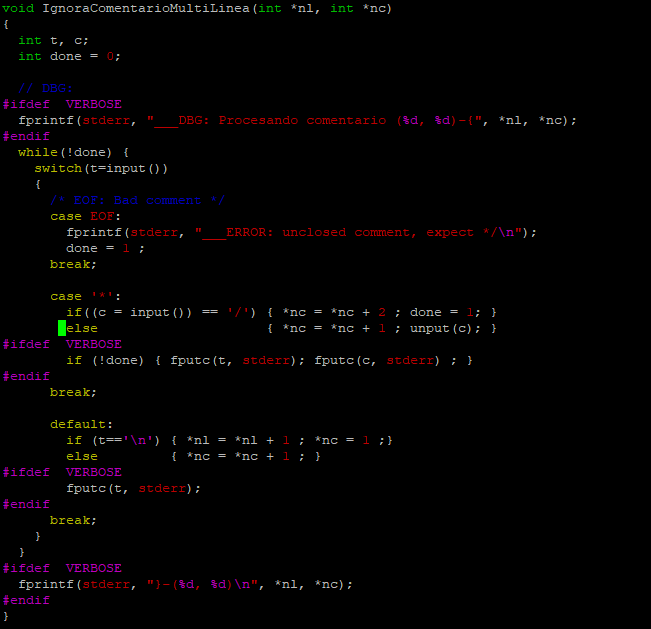
\includegraphics[width=0.65\textwidth]{multi.PNG}}
  \caption{Código del método IgnoraComentarioMultiLinea.}
\end{figure}

\noindent Cabe remarcar que he optado por esta solución porque la considero más completa que aquella que solo contemple comentarios de una línea. En caso de implementar esa solución bastaría con que cada vez que el analizador se encontrase un patrón $"//"$ se ejecutase el método \textit{IgnoraComentario(&nlin, &ncol)} e ignorar todo aquello que se encontrase hasta el primer salto de línea (\textit{$\textbackslash n$}). En el caso de ignorar el comentario multilínea se ignora hasta encontrar el patrón $"*/"$.

\subsection{Operadores}

\begin{itemize}
    \item \textbf{Aritméticos:} '+' (suma), '-' (resta, cambio de signo), '*' (producto), '/' (división),'\%' (división entera), \^ (potencia).
     \item \textbf{Lógicos:} '>' (mayor), '<' (menor), '>=' (mayor o igual)', '<=' (menor o igual), '=='
(igual), '!=' (diferente), ' !' (not), '\&\&' (and), '||' (or).
    \item \textbf{Asignación:} '=' que se empleará en las sentencias de asignación.
\end{itemize}

\noindent Para representar dichos elementos hay que añadir en las definiciones del \textit{lexer} lo siguiente: 

\begin{minted}{bash}

    OP1       ([-+*/=<>?:()!^])
    OP2       ("=="|"!="|"<="|">="|"&&"|"||")

\end{minted}

\noindent Como podemos ver he realizado dos distinciones entre todas las operaciones dando lugar a dos comportamientos distintos en función si se encuentra el patrón \textit{OP1} o \textit{OP2}.

\begin{figure}[H]
  \centering
    \fbox{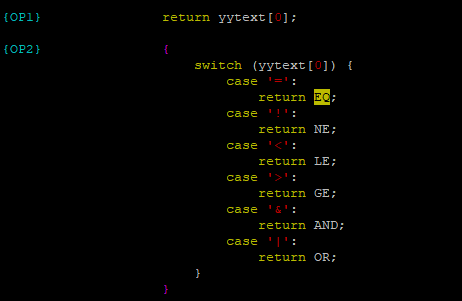
\includegraphics[width=0.65\textwidth]{op.PNG}}
  \caption{Acciones en función de las operaciones.}
\end{figure}

\newpage

\subsection{Errores}

\noindent Como bien se indica al comienzo del enunciado, en caso de que el intérprete lea cualquier carácter que no se corresponda con las reglas expuestas anteriormente será señalado como un error sintáctico y se indicará su localización. Es por esto que en la parte intermedia del archivo \textit{Lex} se definirá el siguiente patrón (usando el punto porque representa cualquier caracter, se dispone la última para así solo activarse una vez que ninguno de los demás patrones se haya disparado):

\begin{minted}{bash}

.   {
        prError(yylineno,"Carácter inesperado en la entrada: \%c [\%d]\n",
        yytext[0],yytext[0],NULL);
    }

\end{minted}

\section{Especificaciones sintácticas}

\noindent En esta parte de la práctica, de todas las especificaciones requeridas, he conseguido implementar las siguientes: 

\begin{itemize}
    \item \textbf{Asignación.}
    \item \textbf{Sentencia vacía.}
    \item \textbf{Sentencia bloque.}
    \item \textbf{Funciones de entrada y salida: read y write.}
    \item \textbf{Sentencia condicional if/else.}
    \item \textbf{Bucle condicional while.}

\end{itemize}

\subsection{Asignación}

\noindent Para que una asignación sea reconocida por el intérprete del lenguaje \textit{P} tiene que constar de un identificador en la parte izquierda de la igualdad ('=') y una expresión en la parte derecha. Obviamente puede ir seguido de cero o más caracteres de separación. Para conseguir esto es necesario añadir lo siguiente en el archivo \textit{pcc.y}:

\begin{minted}{bash}

%token <s>  IDENT PUNTOYCOMA
%type  <s>  ternary 

%%

statement
  :  IDENT '=' ternary PUNTOYCOMA
    {
      $$.flag = fAST;
      $$.u.ast = mkNd('=', mkSlf(IDENT,$1.u.vStr), $3.u.ast);
    }

\end{minted}

\noindent En donde tanto IDENT (mostrado ya anteriormente) como PUNTOYCOMA ($";"$) están definidos en el analizador léxico. Cabe resaltar que el ';' no sería necesario definirlo y bastaría con ponerlo directamente entre comillas simples. En el lexer además tendríamos que definir la acción a realizar cada vez que se encuentren dichos patrones, en caso de punto y coma no hacer nada, mientras que si se encuentra un patrón concordante con IDENT sería lo siguiente:

\begin{minted}{bash}


{PUNTOYCOMA}            {
                        ++yylineno;
                        return PUNTOYCOMA;
                    }


{IDENT}             {
                        unsigned i = 0;
                        int r=-1;
                        char *res;

                        lower(yytext);

                        while (i<KWLEN && r<0) {
                            if ((r=strcmp(keywords[i],yytext))==0) return keycodes[i];
                            ++i;
                        }

                        yyStr(yylval)=sdup(yytext);
                        yyFlag(yylval)=fIDENT;

                        return IDENT;
                    }

\end{minted}

\noindent Además de esto, las \textit{reglas de producción} asociadas a \textit{ternary} son expresiones (IDENT, SIN, TAN, FLOAT...). Dichas asociaciones y reglas de producción pueden verse en el archivo \textit{pcc.y}. \\
\noindent En el fragmento de código mostrado anteriormente vemos también cómo se va construyendo el \textit{árbol de sintaxis abstracta (AST)} en el que el nodo raíz es el '=', el hijo izquierdo es IDENT y el derecho \textit{ternary}. Para acceder a los valores de dichos registros utilizamos el símbolo \$. Para ir construyendo dicho árbol incluímos en el fichero \textit{astree.c} la parte correspondiente a '=':

\begin{minted}{bash}

case '=':
    insertModify( sv(left(root)), expr(right(root)) );
    break;

\end{minted}

\newpage

\subsection{Sentencia vacía}

\noindent Tal y como ha sido presentada la sentencia vacía en el enunciado entiendo el concepto como una sentencia que tan solo consta de ';'. Para implementar esto basta con añadir que los elementos de un programa pueden ser o bien sentencias seguidas de un salto de línea, o solo un salto de línea o solo un punto y coma. Esto es añadido en el fichero \textit{yacc}.


\subsection{Funciones de entrada y salida}

\subsubsection{Write}

\noindent Esta función venía ya implementada por Dusan Kolár, tan solo requería cambiar de nombre de \textit{print} a \textit{write}. Este hecho me costó bastante porque no recordaba que los \textit{Keywords} y los \textit{Keycodes} tenían que estar ordenados alfabéticamente. A continuación se va a mostrar las correspondientes reglas de producción y su implementación para construir el \textit{AST}:

\begin{figure}[H]
  \centering
    \fbox{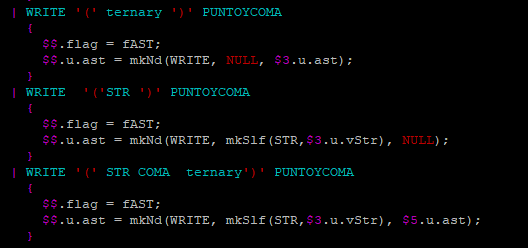
\includegraphics[width=0.75\textwidth]{write.PNG}}
  \caption{Dentro del fichero pcc.y.}
\end{figure}

\begin{figure}[H]
  \centering
    \fbox{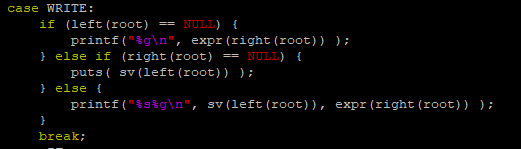
\includegraphics[width=0.75\textwidth]{write2.PNG}}
  \caption{Dentro del fichero astree.c.}
\end{figure}

\newpage

\subsubsection{Read}

\noindent Esta función de entrada puede tomar dos parámetros (separados por una coma) o solo uno. En caso de ser dos parámetros se tratará de un \textit{String} y una variable que almacenará el valor leído. Otra  posibilidad de ejecutar dicha función es sin texto adicional proporcionando un único parámetro al que se le quiere dar valor. Para conseguir esto bastaría con añadir la siguiente \textit{regla de producción} para la variable \textit{statement}:


\begin{figure}[H]
  \centering
    \fbox{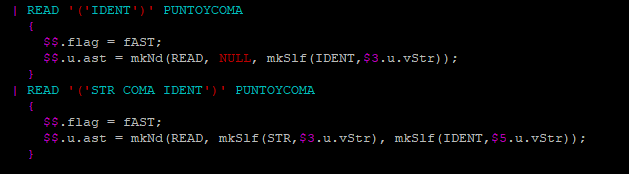
\includegraphics[width=0.75\textwidth]{read.PNG}}
  \caption{Dentro del fichero pcc.y.}
\end{figure}

\noindent Al igual que en el caso de PUNTOYCOMA el token COMA podría haberse puesto literalmente entre comillas simples (en el lexer ha tenido que ser definido, tampoco se realiza nada cuando el intérprete lo lee). Podemos ver en ambos casos cómo se van construyendo el \textit{AST}. A continuación se va a mostrar la parte del \textit{switch} correspondiente, encontrándose éste en el fichero \textit{astree.c} el cual es el encargado de construir el árbol:

\begin{figure}[H]
  \centering
    \fbox{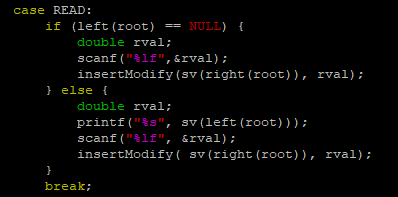
\includegraphics[width=0.65\textwidth]{read2.PNG}}
  \caption{Funcionamiento de read.}
\end{figure}

\noindent Como vemos en la imagen superior, en caso de que el hijo izquierdo sea nulo significa que estamos en el caso de un único parámetro (no hay String) por lo que mediante las funciones \textit{scanf} y \textit{insertModify} se almacena el valor que se encuentra en el hijo derecho. En la situación de ser dos parámetros la única diferencia reside en que, además de lo ya comentado, se imprime el hijo izquierdo (el String).


\newpage

\subsection{If-else}

\noindent La estructura del \textit{if-else} implementada es la requerida en el enunciado de la práctica, siendo la regla de producción construida la siguiente:

\begin{minted}{bash}


ifstmt
   : IF  '(' ternary ')' CORCHETES EOL  body EOL   CORCHETES
        {
        $$.flag = fAST;
        $$.u.ast = mkNd(IF, $3.u.ast,$7.u.ast);
        }
   | IF  '(' ternary ')' CORCHETES EOL  body EOL   CORCHETES ELSE CORCHETES EOL body EOL CORCHETES
        {
        $$.flag = fAST;
        $$.u.ast = mkNd(ELSE, $3.u.ast,mkNd(';',$7.u.ast,$13.u.ast));
        }
        ;
        

body
        : statement
                {
                $$.flag = fAST;
                $$.u.ast = appR(';', NULL, $1.u.ast);
                }
        | body EOL statement
                {
                $$.flag = fAST;
                $$.u.ast = appR(';', $1.u.ast, $3.u.ast);
                }
                ;

\end{minted}

\noindent En donde \textit{ifstmt} se encuentra en las regla correspondiente a \textit{statement}. Podemos observar cómo se definen dos reglas distintas, una para el caso \textit{if} simple y otra para el caso \textit{if-else}, además también es necesario definir un cuerpo (\textit{body}) para que pueda haber más de una sentencia. La implementación correspondiente para construir el árbol es la siguiente:

\begin{figure}[H]
  \centering
    \fbox{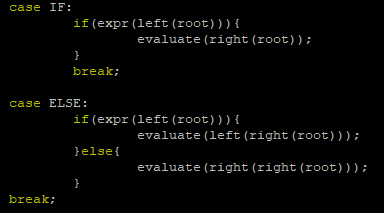
\includegraphics[width=0.65\textwidth]{ifelse.PNG}}
  \caption{Fichero astree.c}
\end{figure}

\noindent Se puede obsrvar cómo en el caso del \textit{if} solo se evalua la expresión del hijo izquierdo, en caso de ser cierto se evaluan las sentencias del hijo derecho. En el caso de usar \textit{else} necesitamos construir un  nivel más del árbol para considerar la alternativa de evaluar las sentencias del cuerpo correspondiente al \textit{else}.

\subsection{While}

\noindent Una vez implementado el \textit{if-else} realizar esto sería bastante simple, la explicación al respecto es bastante similar por lo que no entraré muy en detalle en el código mostrado a continuación.

\begin{minted}{bash}

whilestmt
        : WHILE '(' ternary ')' CORCHETES EOL  body EOL  CORCHETES
           {
           $$.flag = fAST;
           $$.u.ast = mkNd(WHILE, $3.u.ast, $7.u.ast);
           }
           ;
           
\end{minted}

\noindent Al igual que en el caso anterior \textit{whilestmt} es una regla de producción de \textit{statement} y también tenemos que hacer uso de la variable \textit{body}.

\begin{figure}[H]
  \centering
    \fbox{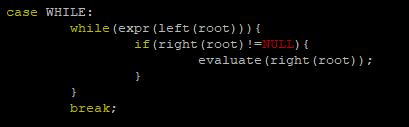
\includegraphics[width=0.65\textwidth]{while.PNG}}
  \caption{Fichero astree.c}
\end{figure}


\subsection{Funciones predefinidas}

\noindent En este apartado se quiere dar soporte tanto a funciones trigonométricas (\textit{sin, cos tan, asin, acos y atan}) como funciones matemáticas (\textit{log, log10, exp, ceil y floor}). En esta situación la implementación de todas es análoga por lo que solo se va a mostrar el caso de una.\\
Para que e intérprete consiga reconocer el seno de un valor es necesario incluir en las \textit{reglas de producción} de expresiones (\textit{expr}) lo siguiente: 

\begin{minted}{bash}

| SIN '(' ternary ')'
    {
      $$.flag = fAST;
      $$.u.ast = mkNd(SIN,$3.u.ast,NULL);
    }

\end{minted}

\noindent Podemos ver cómo se reconoce el término SIN y cómo se construye el árbol con el hijo \textit{ternary}. Una vez reconocido este patrón es necesario implementar en \textit{astree.c} el correspondiente caso dentro del switch tal que se devuelva el cálculo de aplicar la función seno a lo que esté conteniendo \textit{ternary}.

\begin{minted}{bash}
case SIN:
    return sin(expr(left(root)) );
\end{minted}

\noindent Cabe recordar que SIN ha tenido que ser definida como término en \textit{pcc.y} y además como palabra clave en el analizador léxico (al igual que el resto de palabras claves usadas hasta el momento: \textit{read, cos, sin, ...}).

\subsection{Expresiones}

\noindent Lo referido a este apartado, tanto como las propiedades de asociación (por la izquierda, por la derecha...), como las reglas de producción, como la implementación para construir el árbol se ha tomado la solución dado por Dusan por lo que no se incluirán aquí.

\newpage

\section{Extensiones}

\noindent De todas las extensiones que se proponían he decidido realizar solo una debido a que nos encontramos en la etapa final del curso y hay demasiada carga de trabajo del resto de asignaturas. He decidido implementar el \textit{for}.

\subsection{For}

\noindent Cabe destacar que esta opción me ha costado más implementarla debida a que la sentencia cuenta con más elementos por lo que será necesario construir un árbol de mayor profundidad que en los casos anteriores. Antes de nada cabe destacar que mi implementación del \textit{for} no sigue exactamente la misma sintaxis que la pedida en el enunciado, esto es debido a cómo había implementado las asignaciones con los puntos y coma. Para que el intérprete lo acepte tiene que tener el siguiente formato:

\begin{minted}{bash}

for(i=0;i=i+1;i<10){
    // sentencias
}
\end{minted}

\noindent En lugar de lo requerido:

\begin{minted}{bash}

for(i=0;i<10;i=i+1){
    // sentencias
}
\end{minted}

\noindent En el archivo \textit{yacc} tendríamos que introducir la siguiente regla:

\begin{minted}{bash}

forstmt
        : FOR '(' statement statement ternary')' CORCHETES EOL body EOL CORCHETES
           {
           $$.flag = fAST;
           $$.u.ast = mkNd(FOR,$3.u.ast,mkNd(';',$4.u.ast,mkNd(';',$5.u.ast,$9.u.ast)));
           }
           ;
\end{minted}

\noindent Siendo \textit{forstmt} cuerpo de la cabecera \textit{statement}. Podemos observar cómo la construcción del \textit{AST} es mucho más compleja debido a su profundidad. Para implementarlo incorporamos el código siguiente en el que se realiza la asignación de la variable que guía el bucle, se comprueba la condición del bucle y si se cumple se evalua el cuerpo y posteriormente se actualiza el valor de la variable.

\begin{figure}[H]
  \centering
    \fbox{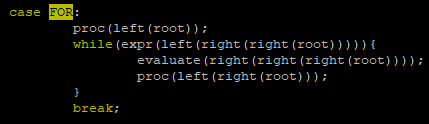
\includegraphics[width=0.65\textwidth]{for.PNG}}
  \caption{Fichero astree.c}
\end{figure}


\section{Ejecución}

\noindent Remarcar que solo existe un fichero de prueba en el que se realizan las comprobaciones para todas las funcionalidades implementadas en la práctica. Además de esto se ha realizado un fichero \textit{bash} en el que se crea el intérprete que posteriormente habrá que ejecutar con el fichero de prueba llamado \textit{test/ejemplo}. El contenido del \textit{bash} es el siguiente:

\begin{minted}{bash}

bison --defines -v pcc.y -o pcc.c
flex -o inter05.lex.c pcc.l
gcc pcc.c inter05.lex.c symtab.c stduse.c astree.c  -o x_pcc -lm


\end{minted}

\bigskip
\begin{thebibliography}{9}

\bibitem{campus} 
Valentín Cardeñoso Payo. \textit{Documentación de la asignatura Gramáticas y Lenguajes Formales}. [\textit{UVA}]
 
\bibitem{dusan} 
Diapositivas y conferencia de Dusan Kolár. [Universidad de Brno]


\end{thebibliography}


\end{document}
